\documentclass[../main.tex]{subfiles}

\begin{document}

% \definecolor{light-gray}{gray}{0.9}
% \newcommand{\code}[1]{
% 	\colorbox{light-gray}{\texttt{#1}}
% }

The dataset consists of 272 images of animals and matching images of the segmentation masks. The dataset was created by students of the SUT by finding relevant images online and tagging them by hand.
The images are of various sizes and use different file extensions - mostly \code{.jpg} (226 files), but also \code{.png} (40 files) and \code{.jpeg} (6 files).

An example image-mask pair taken from the dataset can be seen on figure \ref{fig:dataset:image-mask-example}.

\begin{figure}[htb]
	\centering
	\begin{subfigure}{0.45\textwidth}
		\centering
		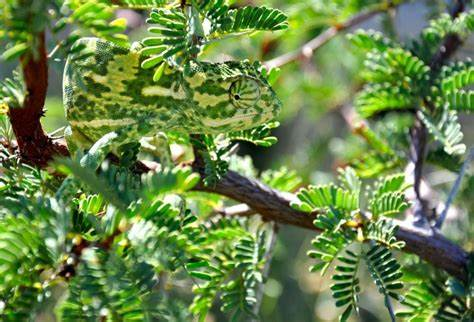
\includegraphics[width=0.95\linewidth]{dataset/example_image.jpg}
		\caption{Camouflaged animal}
	\end{subfigure}
	\begin{subfigure}{0.45\textwidth}
		\centering
		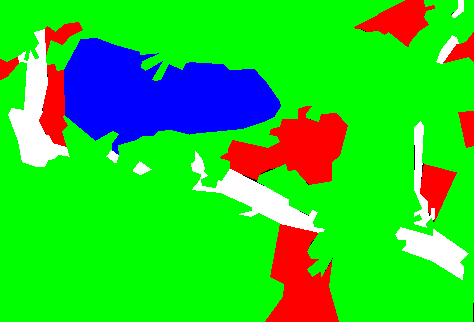
\includegraphics[width=0.95\linewidth]{dataset/example_mask.png}
		\caption{Corresponding mask}
	\end{subfigure}

	\caption{Example of an image-mask pair taken from the dataset}
	\label{fig:dataset:image-mask-example}

\end{figure}


\end{document}